\chapter{Program a jeho realizace}
Nejefektivnější se mi zdálo psát program v programovacím prostředí \textit{Visual Studio Code} \cite{Visualstudio}, se kterým jsem měla nejvíc zkušeností. 

Jedná se o bezplatný editor zdrojového kódu, vhodný pro programování v jakémkoliv programovacím jazyce, bez potřeby přepínání mezi editory. \textit{Visual Studio Code} má podporu programovacích jazyků jako jsou: Python, Java, C++, Javascript a mnoho dalších. 

Kromě \textit{Visual Studio Code} bylo při realizaci použito i jeho plug-in rozšíření s názvem \textit{PlatformIO} \cite{platformio}, což je soubor knihoven, kompatibilních s knihovnami od \textit{Robotárny}. \textit{Robotárna} toto rozšíření využívá a programuje v něm už léta.  Je skvěle kompatibilní s knihovnami \textit{Arduina} a~knihovnami \textit{SmartLeds}, které byly použity z důvodu jejich jednoduchosti a intuitivnosti při programování LED.
%Bylo použito vs. Požila jsem????



\section{Diagram programu }

\begin{figure}[htbp]
	\centering
	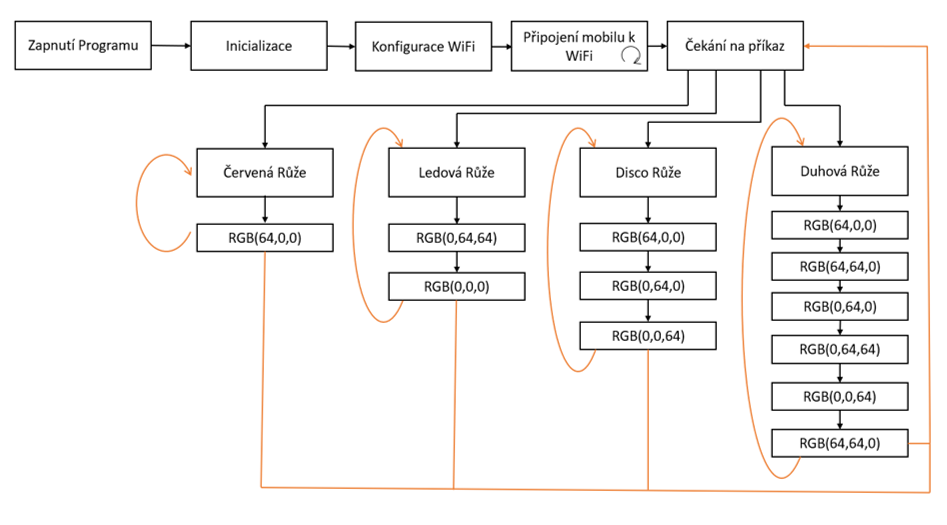
\includegraphics[width=1\textwidth]{img/04prog/Diagramprogramu.png}
	\caption{Blokový diagram programu}
	%	\label{fig:install-sdk-3}
\end{figure}

Tento blokový diagram ukazuje příkazy programu, jak jsou naprogramovány od spuštění (zmáčknutím tlačítka se začne provádět inicializace) až do vypnutí (proces vypnutí může být zahájen v~jakékoliv části programu, stačí jen sepnout tlačítko, a tím přerušit dodávku elektrické energie). 
\newpage

V dalších kapitolách jsou podrobněji rozepsané některé části programu.


\section{Inicializace}
V této části programu se začnou načítat a spouštět veškeré knihovny zahrnuté v programu. Mezi nimi je i soubor \textit{layout.hpp}, který byl vytvořen a uložen v předchozí kapitole. Jsou zde také informace, který je řídící pin LED pásku a kolik LED bude pásek obsahovat.


\section{Konfigurace WiFi a připojení mobilního telefonu k~Wifi}
%konfigurace = nastavení
V těchto částech programu se kompletně nastaví a zapne vysílaný WiFi signál. Nastaví se jméno a heslo, pod kterými se na WiFi lze připojit. V našem případě se jedná o WiFi s~názvem LEDLED a heslem „ledkyledky“. Dále se nastaví vlastník zařízení, název zařízení, čas kompilace zařízení a za pomoci souboru \textit{layout.hpp} sa nastaví podoba ovládacího panelu v mobilním telefonu. 

Po připojení mobilního telefonu na WiFi a zobrazení ovládacího panelu v aplikaci \textit{RBController} už program v \textit{ESP32-DevKitC} jenom čeká na jeden z naprogramovaných příkazů, aby ho mohl provést.
%Inicializace zařízení? 


\section{Příkazy}
Příkazy se v tomhle případě rozumí naše 4 nadefinovaná tlačítka, které jsme si vytvořili v~předchozí kapitole. Každé z těchto tlačítek má v programu přidělenou vlastní funkci, kterou po zmáčknutí provede.

Barva světel je naprogramovaná pomocí RGB spektra. V některých případech se jedná o~jednu prostou barvu, v jiných o donekonečna se opakující se různobarevný cyklus. 

Tlačítka a jejich příkazy: 
\begin{itemize}
	\item \textbf{Červená růže} – barva LED se nastaví na RGB(64,0,0) – tedy červenou barvu. Touto barvou zařízení září po celou dobu. 
	
	\item \textbf{Ledová růže} – jedná se o cyklický barevný přechod. Světle modré světlo se pomalu rozsvěcuje a poté zhasíná, čímž vytváří pulzující dojem magického předmětu. 
	
	\item \textbf{Disko růže} – cyklus, ve kterém se zběsile střídají 3 barvy (červená, modrá a zelená). Bylo původně spíše myšleno jako recese a nachází se zde pro zastoupení různorodosti barevných kombinací. 
	
	\item \textbf{Duhová růže} – mnohobarevný cyklus, který projde celým barevným spektrem. 
\end{itemize}


Veškeré příkazy jsou provedeny pomocí nadefinované funkce \textit{SetLedAll}, která při zadání tří čísel automaticky veškeré LED na pásku nastaví danou RGB barvu a není potřeba každou jednotlivou LED nastavovat samostatně. 

Při programovaní LED pásku nebyla použita maximální intenzita LED pásku. Rozsah RGB je sice od 0 do 255, ale při použití plné intenzity 255 bylo světlo z LED až moc jasné a po delší práci a koukání se na barvy z něj mě začaly bolet oči a hlava. Proto byla světelná intenzita LED pásku snížena na čtvrtinu. 
\newpage